\chapter{Week13}

\section{Monday}\index{Monday_lecture}
\[\dot{\X}=f(\X)
\]
\begin{proposition}
Suppose a solution $\X(t)\rightarrow \xi$ as $t\rightarrow\infty$. Then $f(\xi)=0$
\end{proposition}
\begin{proof}
\begin{figure}[H]
\centering
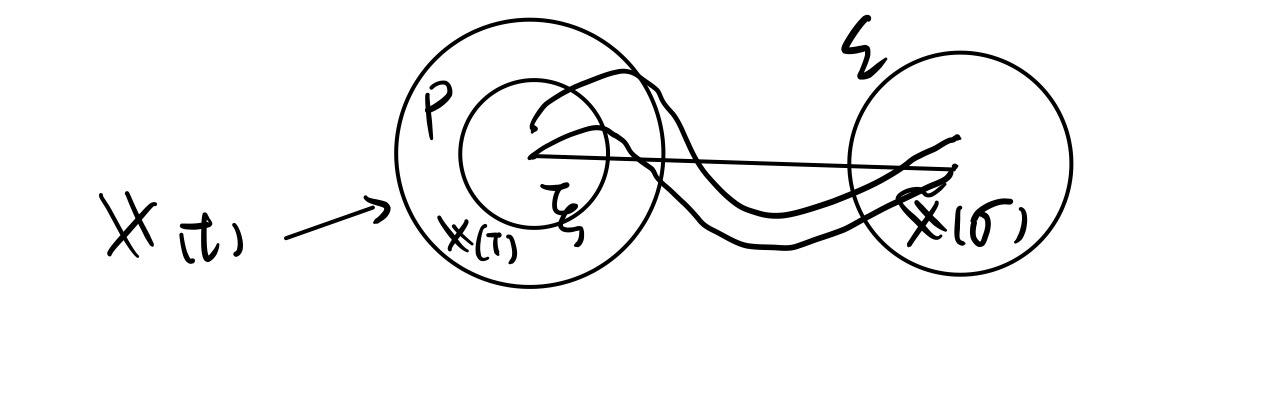
\includegraphics[width=10cm]{week13}
\end{figure}
Suppose Not, i.e. suppose $f(\xi)\neq0$\\
Consider IVP $\begin{cases}\dot{\tilde{\X}}=f(\tilde{\X})\\\tilde{\X}(0)=\xi\end{cases}$
\[f(\xi)\neq0\Rightarrow\tilde{\X}(\delta)\neq\xi \text{ for some } \delta>0
\]
Let $\varepsilon=||\xi-\tilde{\X}(\delta)||>0$ as $\X(t)\rightarrow\xi$ as $t\rightarrow\infty$
$\Rightarrow$ $\exists T$ s.t. $||\X(t)-\xi||<\frac{\varepsilon}{3}$ $\forall t>T$\\
$\exists \rho>0$ s.t. $\forall ||\X^*(0)-\xi||<\rho \Rightarrow ||\X^*(\delta)-\tilde{\X}(\delta)||<\frac{\varepsilon}{3}$ when $\X^*$ is a solution for $\dot{\X}=f(\X)$ (Continuous dependence on IV) \\
$\X(t)\rightarrow\xi\Rightarrow\exists S>0$ s.t. $||\X(t)-\xi||<min\{\rho,\frac{\varepsilon}{3}\}$\\
$\forall t\geq\max(S,T)=\bar{T}$
\[||\X(\bar{T}+\delta)-\tilde{\X}(\delta)||<\frac{\varepsilon}{3}\qquad\bar{T}+\delta\geq T
\]
On the other hand $||\X(\bar{T}+\delta)-\xi||<\frac{\varepsilon}{3}$
\end{proof}
\begin{example}
\[\begin{cases}
\dot{x}(t)=ax-bxy-ex^2=x(a-by-ex)\\
\dot{y}=-cy+dxy-fy^2=y(-c+dx-fy)
\end{cases}
\]
where $a, b, c, d, e, f$ are positive constant and $\frac{a}{e}<\frac{c}{d}, x>0, y>0$.
\[x=0 \text{ or } a-by-ex=0 
\]
\[y=0\text{ or } -c+dx-fy=0
\]

Conclusion: all solutions with $x(0)>0, y(0)>0$ will converge to $(\frac{a}{e},0)$ as t $\rightarrow\infty$\\
At $A$ $\begin{cases}\dot{x}=x(a-by-ex)=0\\\dot{y}(-c+dx-fy)<0\end{cases}$, at B $\begin{cases}\dot{x}<0\\\dot{y}=0\end{cases}$
\begin{itemize}
\item All solutions start in iii will enter ii at a later time 
\item All solutions start in ii will enter i at a later time or converge to $(\frac{a}{e},0)$
\item All solutions in i will converge to $(\frac{a}{e},0)$

\end{itemize}


Question what if $\frac{a}{e}>\frac{c}{d}$
\end{example}
\subsection{Poincare-Bandixon Theorem}
Consider $\dot{\X}=f(\X)$, $n=2$ Suppose $\mathbb{R}$ is a bounded closed subset in $\mathbb{R}^2$ which contains no equilibrium of $f(\X)$. If $\exists a $ solution $\X(t)$ which is contained entirely in $R$, then either $\X(t)$ is periodic or its orbit spirals into a simple closed curve.( i.e. the orbit of a periodic solution.) In particular, $\mathbb{R}$ contains a periodic solution.
\begin{example}
\[\ddot{z}+\dot{z}(z^2+2\dot{z}^2-1)+z=0
\]
Let $\dot{z}=y$, $\dot{y}=\ddot{z}=-[\dot{z}(z^2+2\dot{z}^2-1)+z]$.
\[\begin{cases}\dot{z}=y\\\dot{y}=y(1-z^2-2y^2)-z
\end{cases}
\]
\[\frac{d}{dt}(z^2+y^2)=2z\dot{z}+2y\dot{y}=2y^2(1-z^2-2y^2)
\]
\[z^2+y^2=\frac{1}{4}\text{ on } z^2+y^2=\frac{1}{4},\frac{d}{dt}(z^2+y^2)\geq0
\]
\[z^2+y^2=4\text{ on }z^2+y^2=4, \frac{d}{dt}(z^2+y^2)\leq0
\]
P-B theorem $\Rightarrow$ $\exists$ periodic orbit in $[\frac{2}{4}\leq y^2+z^2\leq4]$.
The annular area is chosen arbitrarily. You can choose any circle you like only if it satisfies the condition of the theorem.
\end{example}



